

\documentclass[12pt]{article}

\usepackage[T1]{fontenc}
\usepackage{amsfonts, amsmath, amssymb}
\usepackage{authblk}
\usepackage{multirow}
\usepackage{epsfig}
\usepackage{subfigure}
\usepackage{subfloat}
\usepackage{graphicx}
\usepackage{lscape}
\usepackage{amsmath}
\usepackage{amssymb}
\usepackage{gensymb}


\usepackage{booktabs}
\usepackage{longtable}
\usepackage{verbatim, rotating, paralist}
\usepackage{enumerate}
\usepackage{natbib}
\usepackage{multibib}
\usepackage{pdfsync}
\usepackage{latexsym}
\usepackage{amsthm}

\usepackage{stmaryrd}
\usepackage{dsfont}
\usepackage{hyperref}
\usepackage{bbm}
\usepackage{mathtools}

\usepackage{parskip}
\usepackage{anysize, indentfirst, setspace}
\usepackage[right=2.25cm, left=2.25cm, top=2.25cm, bottom=2.25cm]{geometry}
\usepackage{tikz}
\usetikzlibrary{arrows,shapes,backgrounds,positioning,patterns,decorations.pathreplacing}
\usepackage{epigraph}
\usepackage{csquotes}

\usepackage{appendix}
\usepackage{enumitem}
\usepackage{rotating}


\setlist{nosep}

\renewcommand{\topfraction}{.85}
\renewcommand{\bottomfraction}{.7}
\renewcommand{\textfraction}{.15}
\renewcommand{\floatpagefraction}{.66}
\renewcommand{\dbltopfraction}{.66}
\renewcommand{\dblfloatpagefraction}{.66}



\newcites{sec}{Appendix References}


%-------------------------------BEGIN DOCUMENT-------------------------------%
\begin{document}

\onehalfspacing
\setlength{\parindent}{0.3in}
\setlength{\parskip}{.0in}


\title{The Margins of Mass Incarceration: \\ Evidence from Mid-Century Mississippi}
\author{Adriane Fresh\footnote{\footnotesize Assistant Professor of Political Science; adriane.fresh$@$duke.edu. I wish to thank my army of research assistants for their transcription of the prison rosters.  Their names follow the paper.  Two transcribers in particular, Ellen May Borden and Rhea Abalos, deserve my particular gratitude.  Willian Ashley Vaughan was exceedingly helpful in locating the registers used in the paper.  This research received IRB approval from Duke University, protocol \#2021-0088.}}

\affil{  \vspace*{-.2in} Duke University \\ \vspace{.2in} }  \normalsize

\date{\large Rough draft, \today }


\maketitle
\vspace{.1in}





%----------------------------------ABTRACT----------------------------------%

\begin{abstract}
\bigskip
\noindent The differential incarceration of Black people relative to White people in U.S. state prisons grew from the mid-20th century.  In this paper I investigate the margins of this carceral inequality.  I digitize individual-level intake records on    42,812\unskip~admissions to the Mississippi state penitentiary at Parchman (1941--1981) and to Tennessee's state prisons (1960--1974).  Using a stock-flow accounting of incarceration, I decompose the Black-White gap in incarceration into the contributions of three margins: \emph{entry} (admission), \emph{sentence length}, and \emph{release} (including parole).  I find that entry accounts for between  76\unskip~and  94\unskip\% of the gap in every period, with longer sentences for Black prisoners accounting for most of the remainder.  The racial gap in Mississippi was U-shaped, narrowing to its lowest point in 1957--1964 and widening again after 1965 through differential growth in Black admissions.  That post-1965 growth was concentrated in counties with the largest Black populations, and in property and violent rather than drug offenses.  Within the same county and year, Black prisoners also received longer sentences and, for the same sentence, served longer and were less likely to be paroled---disparities on the release margin that are hidden in aggregate comparisons.
\end{abstract}






%-------------------------------INTRODUCTION---------------------------------%
\newpage
\doublespacing

\noindent The United States incarcerates its Black residents at several times the rate of its White residents, and that disparity is a defining feature of what is now called mass incarceration \citep{Western:2007ut,Alexander:2012tj}.  A large literature locates the roots of this carceral state in the mid-20th century, emphasizing the politics of crime and race in the wake of the Civil Rights movement \citep{Beckett:1997vq,Weaver:2007vr,Murakawa:2014vj,Hinton:2016tb,Beckett:2020vz}.  Political science is increasingly recognizing that carceral institutions \emph{are} political institutions; decisions about who is subject to state punishment, and for how long, are fundamentally political in nature \citep{Gottschalk:2006ub,Lerman:2014wr,Soss:2017wx}.

Yet, despite this understanding of the broad dynamics of incarceration, we still lack a comprehensive understanding of \emph{how} the racial composition of prisons was produced.  The number of people in prison on any day is the product of how many people are admitted, how long they are sentenced to, and how much of that sentence they serve before release.  I refer to these as the \emph{margins} of incarceration.  Each margin is governed by different actors---police, prosecutors and courts at entry; judges, juries and statutes at sentencing; and parole boards, governors and prison administrators at release---and each is subject to distinct political pressures.  A racial gap in incarceration could therefore arise from any one of these margins, and theories of the carceral state make different predictions about which one should matter.  Distinguishing between the margins is not possible with the aggregate prison counts that underlie most historical studies of incarceration \citep{Langan:1991ud,Muller:2012wf}.  It requires individual-level data on admissions, sentences and releases, broken down by race, before and after the purported punitive turn.

In this paper, I set out to answer a set of descriptive questions about how racial inequality in incarceration was produced in the mid-century.  What was the contribution of admissions, sentence length, and release (including parole) to racial inequality in imprisonment?  How did these contributions change over time, and in particular from before to after the Civil Rights era?  To answer these questions I digitize the convict registers of the Mississippi state penitentiary at Parchman, covering the universe of admissions over 1941--1981, and supplement them with intake registers for Tennessee covering most of 1960--1974.  In total, the data comprise    42,812\unskip~admissions, each recording the prisoner's race, age, county of conviction, offense, sentence, dates of sentencing and receipt, and---in most registers---the date and manner of exit from custody.

The choice to study Mississippi was made for two reasons.  First was data availability: Mississippi's registers survive as a near-continuous series with a single penitentiary receiving the state's prisoners.  Second, Mississippi is the archetypal case of the Jim Crow carceral state \citep{Oshinsky:1997up,Mickey:2015vh}.  If the post-Civil Rights growth in racial disparities ran through a particular margin, it should be visible here.  Tennessee provides a useful comparison: an Upper South state, with a much smaller Black population share, whose registers overlap with Mississippi's during the 1960s and early 1970s.

To organize the analysis, I use a simple stock-flow identity.  In a steady state, the number of people in prison per capita equals the admission rate multiplied by the average time served, which in turn is the average sentence multiplied by the fraction of it that is served.  Taking logs, the Black-White ratio of incarceration can be decomposed exactly into the sum of a ratio for each margin.  I estimate this decomposition separately for six periods in Mississippi and two in Tennessee.

I establish four sets of empirical facts.  First, entry is the dominant margin of racial inequality in incarceration throughout the period.  Black admission rates exceeded White admission rates by a factor of between  2.0\unskip~and  3.6\unskip~in Mississippi, and entry accounts for between  76\unskip~and  94\unskip\% of the gap in implied incarceration in every period and state.  Sentence length accounts for the remainder, between   6\unskip~and  23\unskip\%.  Release accounts for approximately none of the aggregate gap.

Second, the racial gap in Mississippi was U-shaped.  The Black-White ratio in implied incarceration fell from 3.95\unskip~in 1941--1948 to 2.32\unskip~in 1957--1964, before rising to 3.78\unskip~by 1977--1980.  The post-1965 increase was driven by entry: Black admissions per 100,000 rose from   46\unskip~on average over 1966--1970 to  129\unskip~in 1980, while White admissions rose from   22\unskip~to   41\unskip.

Third, the post-1965 growth in Black admissions was geographically and substantively specific.  Before 1965, the Black-White admission ratio was \emph{lowest} in the Mississippi counties with the largest Black population shares.  After 1965, it rose most in exactly those counties---from 1.34\unskip~in 1965--1970 to 2.78\unskip~in 1977--1980.  The growth came through property and violent offenses in roughly equal measure.  Drug offenses contributed essentially nothing to the Black-White gap in admissions in Mississippi through 1980.

Fourth, the aggregate decomposition masks disparities on the sentencing and release margins that are visible when comparing Black and White admissions convicted in the same county and year.  In Mississippi, Black prisoners received sentences that were roughly 9 log points longer than those of White prisoners convicted of the same broad offense type in the same county and year, a gap that did not change after 1965.  Holding the sentence itself fixed, Black prisoners served around 6\% longer and were 5 percentage points less likely to leave prison on parole (relative to a White parole share of  24\unskip\%).  In aggregate these release disparities are offset because the share of a sentence that is served falls with sentence length, and Black prisoners had longer sentences.

I present these findings as descriptive patterns of inequality \citep{Kreuzer:2009ic}.  An increasingly rich literature in the social sciences has questioned the extent to which descriptive disparities imply that we can make a causal inference about the \emph{effect} of race---that is, that descriptive disparities are in fact evidence of racial \emph{bias} within carceral institutions.  The registers do not record the evidence before the court, prior arrests that did not result in imprisonment, or the decisions of police and prosecutors that precede admission.  Disparities at entry, in particular, combine differences in offending, policing, prosecution and conviction.  But the decomposition does tell us \emph{where} in the carceral process racial inequality in imprisonment was produced, which is a necessary first step in explaining it.

These findings contribute to the literature on the growth of mass incarceration in the U.S. in three ways.  First, they provide---to my knowledge---the first individual-level decomposition of the margins of racial inequality in incarceration spanning the mid-century punitive turn.  Existing historical work relies on aggregate admissions or prison populations by race \citep{Langan:1991ud,Muller:2012wf,EubankFresh:2021gg,Duxbury:2023em}, or on rich qualitative accounts of particular institutions \citep{Oshinsky:1997up,Lynch:2010rt,Schoenfeld:2018vq}.  Work using comparable individual-level prison registers has focused on earlier periods \citep{10.1017/s002205072610148x}.  Second, they speak to a debate about whether incarceration growth was driven by admissions or by time served.  For the late 20th century, \cite{Pfaff:2017tp} argues that admissions---driven by prosecutors---rather than longer sentences drove growth.  I find that the same holds for racial \emph{disparity} in incarceration in the mid-century South.  Third, the timing and geography of the post-1965 increase in Black admissions accord with accounts that link the carceral state's expansion to White reaction to Black political empowerment \citep{Blalock:1967ud,Weaver:2007vr,EubankFresh:2021gg}, and identify the entry margin as the channel through which that reaction operated.







%----------------------------------SECTION-----------------------------------%
\vspace*{-.1in}
\section*{Race and the Margins of the Carceral State}
\vspace*{-.1in}

\noindent Mass incarceration in the U.S. is typically defined as a phenomenon of the late 20th and early 21st century.  But whereas the magnitude reached unprecedented levels during this latter period, its roots---and particularly the roots of its racial composition---are typically situated earlier \citep{Muller:2012wf,Thompson:2019wo,Beckett:2020vz}.  National series of prison admissions by race show the Black share of admissions growing from the 1920s onward \citep{Langan:1991ud}.  These national series are informative about levels, but they cannot tell us which parts of the carceral process produced the racial composition of prisons.

%% subsection
\subsection*{Three Margins, Three Sets of Institutions}

\noindent The stock of prisoners is produced by three margins.  The \emph{entry} margin is the rate at which people are admitted to prison.  It is the end-point of a chain of decisions---by police about whom to arrest, by prosecutors about whom to charge and what to charge them with, and by courts about whom to convict and whether to imprison rather than fine, suspend or jail them.  The \emph{sentencing} margin is the length of the term imposed.  In the mid-century South, it was shaped by statute, by judges and, in some cases, juries.  The \emph{release} margin is the share of the sentence that is actually served.  It is governed by parole boards, by executive clemency, by earned-time rules and by prison administrators \citep{Oshinsky:1997up,Campbell:2013tw}.

These margins are not equally visible to the public, nor equally accountable to it.  Entry decisions are diffuse, highly local and largely unrecorded, the product of county sheriffs and district attorneys \citep{Pfaff:2017tp}.  Sentencing is more visible, and has been the subject of most later reform.  Release in the mid-century was perhaps the least transparent of all, determined by state-level boards and governors with wide discretion.  This matters because theories of the carceral state differ in which institutions---and thus which margins---they implicate.

%% subsection
\subsection*{Expectations from Existing Accounts}

\noindent Three broad accounts offer different expectations about the margins of racial inequality in incarceration in the mid-century South.

The first emphasizes the labor-control functions of Southern punishment under Jim Crow \citep{Lichtenstein:1996ug,Oshinsky:1997up,Blackmon:2009wo,LeFlouria:2015vj,Muller:2019uv}.  On this account, the incarceration of Black people was tied to the demand for Black labor, both in the state's prison farms and in the private economy.  Where Black labor was most valuable to White landowners---the plantation counties---we might expect \emph{less} formal state imprisonment of Black people, as local and private forms of control substituted for the penitentiary.  We might also expect disparities on the release margin, since clemency and parole were discretionary tools for allocating labor and rewarding deference \citep{Oshinsky:1997up}.

The second account emphasizes White reaction to Black political empowerment.  Racial threat theories argue that the White majority responds to the growing political power of a Black minority with more coercive social control \citep{Blalock:1967ud}.  Applied to the mid-century, this suggests that the Civil Rights movement and the Voting Rights Act prompted a turn towards punitive policy---a ``frontlash'' \citep{Weaver:2007vr}.  \cite{EubankFresh:2021gg} find that states covered by Section 5 of the Voting Rights Act experienced a differential increase in Black prison admissions after 1965, and that this increase varied in proportion to the electoral threat posed by Black voters.  This account predicts that racial disparity should grow after 1965 and should grow most in places where Black people were most numerous.  It is less specific about the margin, but because the relevant actors---sheriffs, prosecutors and local judges---were elected at the county level, it points most naturally to entry.

The third account emphasizes changes in crime and in national crime policy from the late 1960s, including the war on crime and, later, the war on drugs \citep{Beckett:1997vq,Murakawa:2014vj,Hinton:2016tb,Alexander:2012tj}.  This account predicts that disparities should grow through the offense categories targeted by these policies---drug offenses in particular---and potentially through sentence length, as legislatures increased statutory penalties.

These accounts are not mutually exclusive, and the analysis that follows is not a test that adjudicates among them.  Instead, the decomposition identifies which margins changed, when, for which offenses, and where---the empirical facts each account must explain.

%% subsection
\subsection*{Mississippi and Tennessee}

\noindent Mississippi's state penitentiary, Parchman Farm, was a plantation prison in the Yazoo-Mississippi Delta whose history has become emblematic of Jim Crow justice \citep{Oshinsky:1997up}.  Mississippi was also among the most thoroughly authoritarian of the Southern states before 1965 \citep{Mickey:2015vh}, and among those most transformed by the Voting Rights Act.  Tennessee offers a contrast.  It was not covered by Section 5 of the Voting Rights Act, and its Black population share was less than half that of Mississippi.  In both states, Black people were overrepresented among prison admissions throughout the period I study.  The question is through which margins, and how that changed.





%----------------------------------SECTION-----------------------------------%
\vspace*{-.1in}
\section*{Data and Measurement}
\vspace*{-.1in}

\noindent In order to understand how racial disparities in incarceration were produced, it's necessary to have individual data on prisoners.  One needs to know when prisoners were admitted to prison, how long they were sentenced to, and when and how they left, and this data must in turn be broken down by race.  Though many states produced annual and biennial reports with some of this information, these reports rarely cross-tabulate sentences or time served by race, and they are not available consistently over time.

%% subsection
\subsection*{The Convict Registers}

\noindent I digitize the Mississippi state penitentiary's convict registers obtained from the Mississippi Department of Archives and History.\footnote{Catalog record: ``Convict Registers, 1874-1981.'' Contributor: Mississippi Department of Corrections.  Series 1562.  Rolls 15218-15230.}  These are handwritten ledgers in which each prisoner received at Parchman was entered on arrival.  The registers record each prisoner's register number, name, county of conviction, crime, date of sentence, term, date received, age, race, physical description, home, education, occupation, religion, and---in a separate set of columns updated over the prisoner's term---the dates of parole, pardon, discharge, escape or death.\footnote{I transcribe the variables needed to measure the three margins, and a subset of the descriptive variables.  I do not transcribe prisoners' names, register numbers, home addresses (beyond city and state), or physical descriptions other than complexion in the version of the data used here.}  For Tennessee I transcribe the state's prison intake registers on microfilm rolls 39--41 and 45, which cover most admissions between 1960 and 1974 \textbf{[TK: archival citation for the Tennessee registers]}.

The registers were transcribed by two professional transcribers and by a team of student research assistants.  The final Mississippi data comprise    30,899\unskip~admissions, of which    16,345\unskip~were transcribed by a professional transcriber and    13,954\unskip~by student research assistants.  The Tennessee data comprise    11,913\unskip~admissions.  Appendix~\ref{appendix_data} describes how the transcriptions were assembled, how duplicate and misfiled transcriptions were identified and removed, and how dates were parsed and repaired.  Table~\ref{table_data} summarizes the data.



% TABLE: Data
%---------------------------
\begin{table}[t!]\centering \footnotesize
	\caption{The convict registers}\label{table_data}
	\smallskip
	\begin{tabular}{@{\extracolsep{3pt}}l*{9}{c}}
	\noalign{\smallskip}\noalign{\smallskip}\hline\hline\noalign{\smallskip}\noalign{\smallskip}
			& \multicolumn{3}{c}{Admissions} & & Complete & \multicolumn{4}{c}{Share recorded} \\
			\cline{2-4} \cline{7-10} \noalign{\smallskip}
			& All & White & Black & Years & years & Race & Sentence & County & Exit \\
	\noalign{\smallskip}\hline\noalign{\smallskip}
			   Mississippi &    30,899 &    11,418 &    19,299 & 1941--1981 &  29 & 1.00 & 0.98 & 0.99 & 0.84 \\
Tennessee &    11,913 &     7,694 &     4,213 & 1960--1974 &   7 & 1.00 & 0.98 & 1.00 & 0.98 \\
 \\
	\noalign{\vspace*{-.17in}}\hline\hline\noalign{\smallskip}
\multicolumn{10}{p{6.0in}}{\scriptsize  \emph{Notes}: Admissions transcribed from the registers.  \emph{Complete years} are years in which at least 95\% of the year's register pages are transcribed (Appendix~\ref{appendix_coverage}).  \emph{Sentence} is the share of admissions with a parsed term, life or death sentence.  \emph{County} is the share matched to a county of conviction.  \emph{Exit} is the share with a recorded first exit from custody among admissions in registers that record release events. }
\end{tabular}
\end{table}



Two features of the data deserve emphasis.  First, the Mississippi series is close to complete.  Excluding a gap in the surviving microfilm between late 1948 and the end of 1950, the transcribed registers cover at least 87\% of each year's pages in every year from 1959 to 1980, and all pages in most years (Appendix Figure~\ref{figure_coverage}).  Where coverage is incomplete I scale admissions by the inverse of the share of the year covered, and I exclude years in which less than half of the year is covered.  Second, the registers agree closely with the state's own published admission counts.  In years with complete coverage, the number of admissions in the registers is within 1\% of the annual report total in 1960, 1975 and 1979, and the Black share of admissions differs by less than two percentage points in every year I can compare except 1980 (Appendix Table~\ref{table_validate}).\footnote{The register and report totals diverge substantially in 1976 (the register exceeds the report by 25\%) and 1980 (the report is more than twice the register, and reports a much lower Black share).  I cannot determine from the data whether this reflects a change in the reports' definitions---for example, the inclusion of returned parole violators or a change in the reporting year---or missing register pages.}

%% subsection
\subsection*{Measuring the Three Margins}

\noindent \emph{Entry.}  I measure entry as admissions per 100,000 residents of the same race, using county populations by race from the decennial census, interpolated between census years \textbf{[TK: NHGIS citation]}.  Admission dates are the date the prisoner was received at the penitentiary, or the date of sentence where the received date is missing.  Race is recorded by prison officials.  I classify admissions as White or Black; fewer than 0.2\% of Mississippi admissions are recorded as another race and are excluded.

\emph{Sentence length.}  I measure sentence length as the effective term in years: the nominal term (the longest count, or the sum of counts where counts are consecutive) less any portion of the term suspended at sentencing.  In Tennessee, where many sentences are indeterminate, I use the maximum of the range.  I exclude life and death sentences from the measure of sentence length and top-code terms at 50 years.

\emph{Release.}  I measure release by the first exit from custody---by parole, discharge at the expiration of the term, pardon, suspension, or death---and the time from admission to that exit.  The release margin is then the ratio of mean time served to mean sentence, i.e., the fraction of the sentence served.  Two limitations deserve note.  First, some student-transcribed files did not record parole events, so I measure release only in registers that record release events.  Second, the Mississippi registers stopped being updated for many prisoners admitted after 1970, so that exits are under-observed for later cohorts.  Because the exits that \emph{are} recorded for these cohorts are disproportionately quick, the fraction served is biased downwards for these cohorts, which I flag throughout.

%% subsection
\subsection*{Decomposing Racial Inequality in Incarceration}

\noindent To combine the three margins, I use a steady-state stock-flow identity (Little's law).  For race $r$ in a period, the implied number of people in prison per 100,000 is
\begin{equation}
	P_{r} = A_{r} \times S_{r} \times \rho_{r}
	\label{equation_stock}
\end{equation}
where $A_{r}$ is admissions per 100,000 per year (entry), $S_{r}$ is the mean effective sentence in years (sentencing), and $\rho_{r}$ is the mean time served divided by the mean sentence (release).  The ratio of Black to White implied incarceration then decomposes exactly:
\begin{equation}
	\ln \left( \frac{P_{B}}{P_{W}} \right) = \underbrace{\ln \left( \frac{A_{B}}{A_{W}} \right)}_{\text{entry}} + \underbrace{\ln \left( \frac{S_{B}}{S_{W}} \right)}_{\text{sentencing}} + \underbrace{\ln \left( \frac{\rho_{B}}{\rho_{W}} \right)}_{\text{release}}
	\label{equation_decomp}
\end{equation}
The share of the gap due to each margin is its term divided by the left-hand side.  $P_{r}$ is the stock that would be implied if admission rates, sentences and release practices in a period persisted.  It is not the observed prison population, which also reflects admissions in earlier periods and the life-sentenced population.  Its advantage is that it isolates the contribution of each margin to racial inequality among those admitted in a given period.  I estimate equation~\ref{equation_decomp} for six periods in Mississippi (1941--48, 1951--56, 1957--64, 1965--70, 1971--76, 1977--80) and two in Tennessee (1960--66 and 1972--74), and obtain standard errors by bootstrapping admission records within race.\footnote{Because the number of admissions of each race is a full count rather than a sample, the bootstrap standard errors on the entry term reflect only variation in the coverage weights.  They should not be read as capturing uncertainty about the admission rate itself.}






%----------------------------------SECTION-----------------------------------%
\vspace*{-.1in}
\section*{Estimating the Margins of Incarceration}
\vspace*{-.1in}

%% subsection
\subsection*{Trends in the Three Margins}

\noindent I begin by presenting trends in each margin by race and year of admission.  Figure~\ref{figure_entry} presents admission rates.  In Mississippi, Black admission rates exceeded White admission rates in every year.  The two series converged through the 1950s and early 1960s, as White admission rates rose faster than Black admission rates: in 1960, Black admissions were   57\unskip~per 100,000 compared to   26\unskip~for White residents.  Admission rates for both groups then fell in the second half of the 1960s.  From the early 1970s, Black admission rates grew rapidly, reaching   98\unskip~per 100,000 in 1975 and  129\unskip~in 1980; White admission rates grew more slowly, to   41\unskip.  In Tennessee, Black admission rates were higher still, and the gap was wider in 1972--74 than in 1960--66.



%  FIGURE: Entry
%--------------------------------------
\begin{figure}[t!]
	\begin{center}
	\caption{Admissions per 100,000 by race, by year of admission}
	\small \smallskip
		\begin{minipage}{3.1in} \centering \scriptsize \emph{(a) Mississippi} \\
			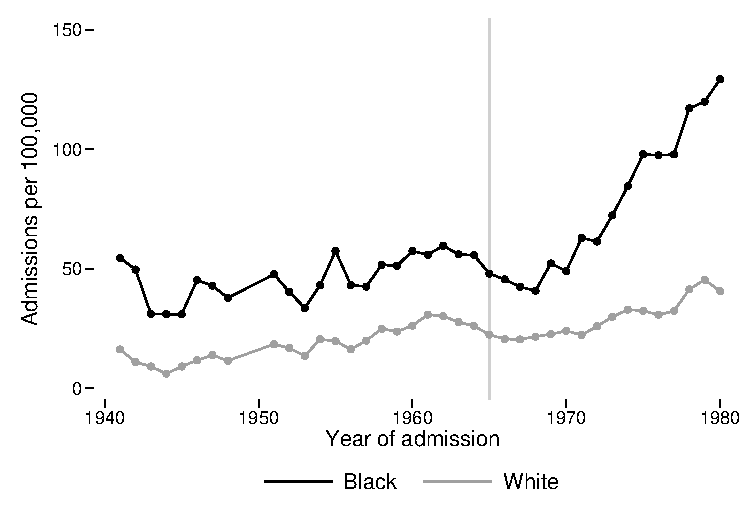
\includegraphics[ width=3.1in,  clip=true,  trim= 0.0in 0in 0in 0in ]{../../../30_output/40_figures/fig_entry_MS.pdf}
		\end{minipage}
		\begin{minipage}{3.1in} \centering \scriptsize \emph{(b) Tennessee} \\
			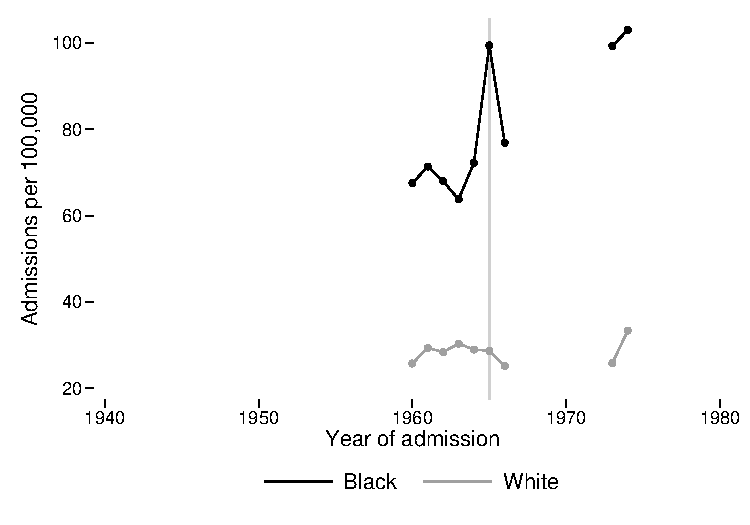
\includegraphics[ width=3.1in,  clip=true,  trim= 0.0in 0in 0in 0in ]{../../../30_output/40_figures/fig_entry_TN.pdf}
		\end{minipage}
	\label{figure_entry}
\end{center}
	\scriptsize{\emph{Source:} Convict registers; census population by race (interpolated). } \\
	\scriptsize{\emph{Notes:} Admissions are scaled by the inverse of the share of the year's register pages transcribed; years with less than half of the year transcribed, and years with fewer than 40 transcribed admissions, are omitted.  The vertical line marks 1965.   }
\end{figure} \normalsize



Figure~\ref{figure_sentence} presents mean effective sentence length.  In both states, Black prisoners received longer sentences than White prisoners in nearly every year.  In Mississippi, mean sentences were relatively stable at three and a half to four and a half years until the late 1960s, and lengthened for both groups thereafter.  Black-White differences in mean sentences in Mississippi ranged from   9\unskip\% in 1941--48 to  26\unskip\% in 1971--76 (Table~\ref{table_levels}).  In Tennessee they were larger, at around a third.



%  FIGURE: Sentence
%--------------------------------------
\begin{figure}[t!]
	\begin{center}
	\caption{Mean effective sentence by race, by year of admission}
	\small \smallskip
		\begin{minipage}{3.1in} \centering \scriptsize \emph{(a) Mississippi} \\
			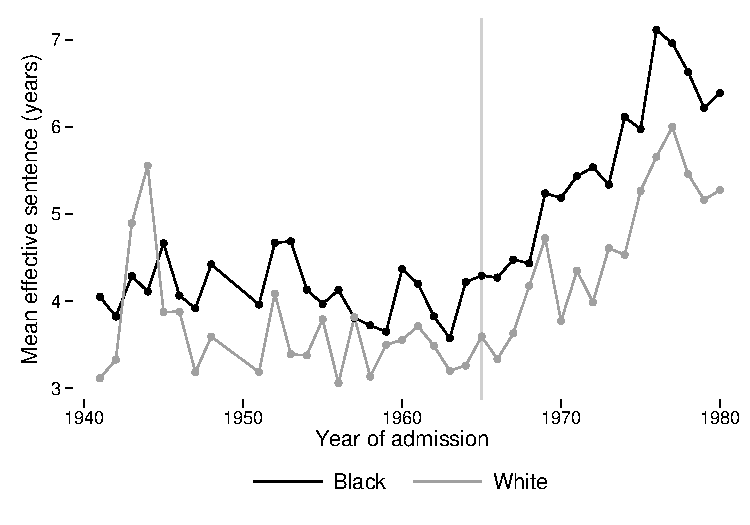
\includegraphics[ width=3.1in,  clip=true,  trim= 0.0in 0in 0in 0in ]{../../../30_output/40_figures/fig_sentence_MS.pdf}
		\end{minipage}
		\begin{minipage}{3.1in} \centering \scriptsize \emph{(b) Tennessee} \\
			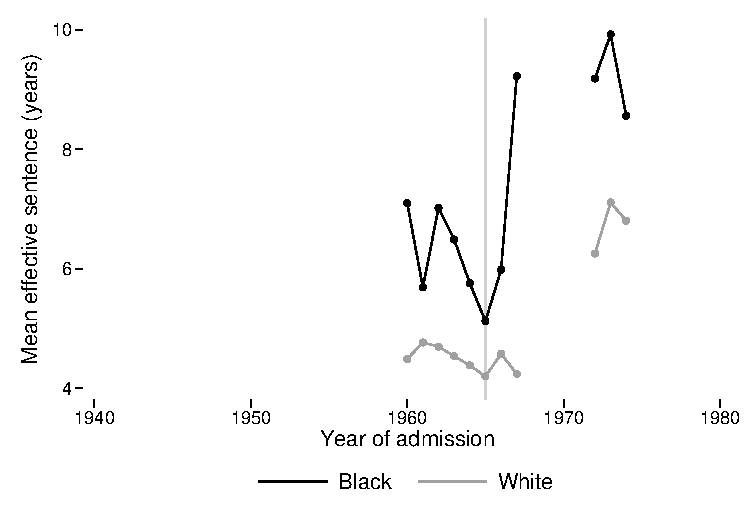
\includegraphics[ width=3.1in,  clip=true,  trim= 0.0in 0in 0in 0in ]{../../../30_output/40_figures/fig_sentence_TN.pdf}
		\end{minipage}
	\label{figure_sentence}
\end{center}
	\scriptsize{\emph{Source:} Convict registers. } \\
	\scriptsize{\emph{Notes:} Mean effective sentence excludes life and death sentences and top-codes terms at 50 years.  In Mississippi, the effective sentence is the nominal term less any suspended portion.  In Tennessee, it is the maximum of an indeterminate range.  The vertical line marks 1965.   }
\end{figure} \normalsize



Figure~\ref{figure_release} presents the fraction of the sentence served.  Before the mid-1960s, prisoners of both races in Mississippi served around two-thirds of their sentence before first exit.  This fell to around one half for cohorts admitted in the late 1960s.\footnote{The fall coincides with the period in which student-transcribed registers make up most of the series, and with gaps in the years for which release events are recorded (Appendix~\ref{appendix_data}).  I have not yet established whether it reflects a change in release practice or a change in which registers record release events.}  For post-1970 cohorts the series continues to fall, but this is in large part an artifact of the registers no longer recording exits for many prisoners (marked by crosses).  Strikingly, the fraction of the sentence served was almost identical for Black and White prisoners in every period and in both states.



%  FIGURE: Release
%--------------------------------------
\begin{figure}[t!]
	\begin{center}
	\caption{Fraction of sentence served by race, by year of admission}
	\small \smallskip
		\begin{minipage}{3.1in} \centering \scriptsize \emph{(a) Mississippi} \\
			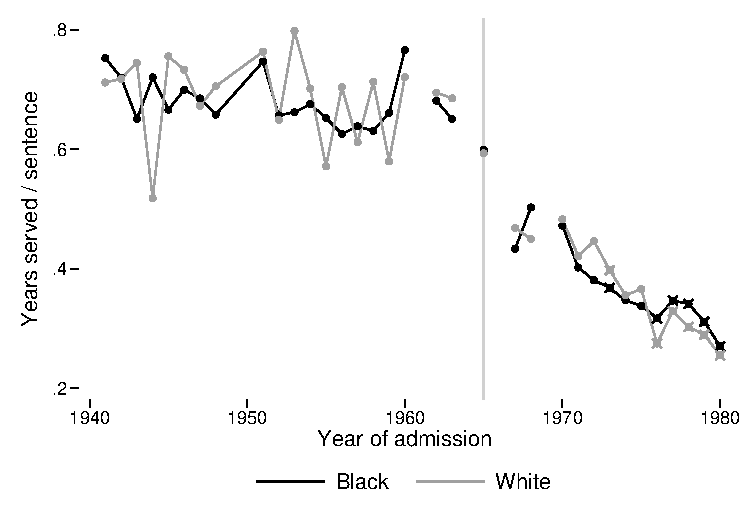
\includegraphics[ width=3.1in,  clip=true,  trim= 0.0in 0in 0in 0in ]{../../../30_output/40_figures/fig_release_MS.pdf}
		\end{minipage}
		\begin{minipage}{3.1in} \centering \scriptsize \emph{(b) Tennessee} \\
			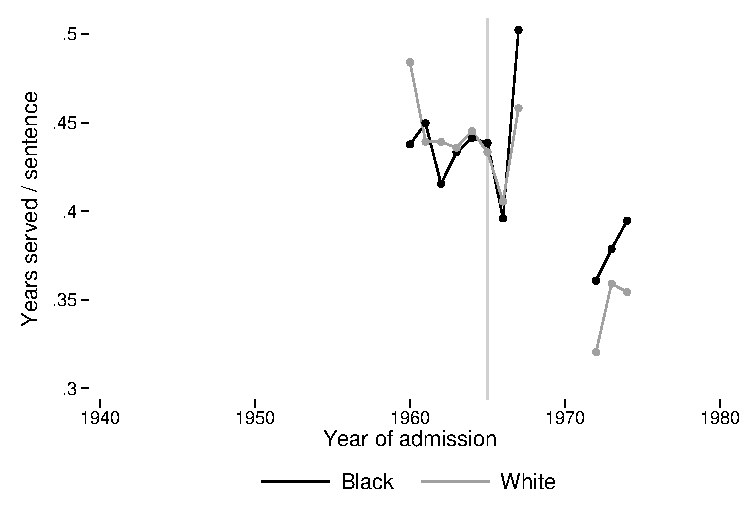
\includegraphics[ width=3.1in,  clip=true,  trim= 0.0in 0in 0in 0in ]{../../../30_output/40_figures/fig_release_TN.pdf}
		\end{minipage}
	\label{figure_release}
\end{center}
	\scriptsize{\emph{Source:} Convict registers. } \\
	\scriptsize{\emph{Notes:} Mean years from admission to first exit divided by mean effective sentence, among admissions with a recorded exit in registers that record release events.  Cohorts with fewer than 30 such admissions are omitted.  Crosses mark cohorts in which fewer than 85\% of admissions have a recorded exit; for these cohorts only quicker exits are observed and the ratio is biased downwards.  The vertical line marks 1965.   }
\end{figure} \normalsize



% TABLE: Levels
%---------------------------
\begin{table}[t!]\centering \footnotesize
	\caption{The three margins of incarceration by race and period}\label{table_levels}
	\smallskip
	\begin{tabular}{@{\extracolsep{4pt}}l*{8}{c}}
	\noalign{\smallskip}\noalign{\smallskip}\hline\hline\noalign{\smallskip}\noalign{\smallskip}
			& \multicolumn{2}{c}{Entry} & \multicolumn{2}{c}{Sentencing} & \multicolumn{2}{c}{Release} & \multicolumn{2}{c}{Implied stock} \\
			& \multicolumn{2}{c}{$A_{r}$} & \multicolumn{2}{c}{$S_{r}$} & \multicolumn{2}{c}{$\rho_{r}$} & \multicolumn{2}{c}{$P_{r}$} \\
			\cline{2-3} \cline{4-5} \cline{6-7} \cline{8-9} \noalign{\smallskip}
			& White & Black & White & Black & White & Black & White & Black \\
	\noalign{\smallskip}\hline\noalign{\smallskip}
			   Mississippi 1941--48 & 11.1 & 40.5 & 3.81 & 4.14 & 0.69 & 0.69 & 29.4 & 116.2 \\
Mississippi 1951--56 & 17.6 & 44.2 & 3.46 & 4.25 & 0.70 & 0.67 & 42.5 & 126.3 \\
Mississippi 1957--64 & 26.3 & 53.7 & 3.45 & 3.93 & 0.66 & 0.66 & 60.2 & 139.7 \\
Mississippi 1965--70 & 22.0 & 46.4 & 3.89 & 4.66 & 0.49 & 0.51 & 41.9 & 110.3 \\
Mississippi 1971--76 & 29.1 & 79.7 & 4.79 & 6.02 & 0.36$^{\dagger}$ & 0.35$^{\dagger}$ & 50.6 & 167.6 \\
Mississippi 1977--80 & 40.0 & 116.2 & 5.41 & 6.51 & 0.30$^{\dagger}$ & 0.32$^{\dagger}$ & 63.9 & 241.5 \\
\noalign{\smallskip}
Tennessee 1960--66 & 28.1 & 74.3 & 4.52 & 6.04 & 0.44 & 0.43 & 55.7 & 192.7 \\
Tennessee 1972--74 & 29.7 & 101.2 & 6.92 & 9.35 & 0.35 & 0.38 & 72.8 & 362.6 \\
 \\
	\noalign{\vspace*{-.17in}}\hline\hline\noalign{\smallskip}
\multicolumn{9}{p{6.2in}}{\scriptsize  \emph{Notes}: $A_{r}$ is admissions per 100,000 residents of race $r$ per year, scaled for coverage.  $S_{r}$ is the mean effective sentence (years) among non-life, non-death admissions, top-coded at 50.  $\rho_{r}$ is mean years to first exit divided by mean sentence among admissions with a recorded exit, in registers that record release events.  $P_{r}=A_{r} \times S_{r} \times \rho_{r}$ is the implied steady-state number in prison per 100,000 (equation~\ref{equation_stock}).  $^{\dagger}$ fewer than 85\% of admissions have a recorded exit; $\rho_{r}$ is biased downwards. }
\end{tabular}
\end{table}



%% subsection
\subsection*{Decomposing the Racial Gap}

\noindent Table~\ref{table_decomp} and Figure~\ref{figure_decomp} present estimates of equation~\ref{equation_decomp}.  In every period and in both states, entry accounts for the large majority of the racial gap in implied incarceration---between  76\unskip~and  94\unskip\%.  The sentencing margin accounts for between   6\unskip~and  23\unskip\%, and the release margin contributes approximately nothing, with estimates that are small, of inconsistent sign, and not distinguishable from zero in most periods.



% TABLE: Decomposition
%---------------------------
\begin{table}[t!]\centering \footnotesize
	\caption{Decomposition of the Black-White gap in implied incarceration}\label{table_decomp}
	\smallskip
	\begin{tabular}{@{\extracolsep{5pt}}l*{6}{c}}
	\noalign{\smallskip}\noalign{\smallskip}\hline\hline\noalign{\smallskip}\noalign{\smallskip}
			& Ratio & $\ln$ ratio & \multicolumn{3}{c}{Contribution of} & Entry \\
			\cline{4-6} \noalign{\smallskip}
			& $P_{B}/P_{W}$ & (total) & Entry & Sentencing & Release & share (\%) \\
	\noalign{\smallskip}\hline\noalign{\smallskip}
			   Mississippi 1941--48 & 3.95 & 1.37 & 1.29 & 0.08 & -0.00 &  94 \\
 & & (0.042) & (0.010) & (0.048) & (0.043) & \\
Mississippi 1951--56 & 2.97 & 1.09 & 0.92 & 0.20 & -0.04 &  85 \\
 & & (0.035) & (0.009) & (0.033) & (0.030) & \\
Mississippi 1957--64 & 2.32 & 0.84 & 0.72 & 0.13 & -0.00 &  85 \\
 & & (0.035) & (0.001) & (0.028) & (0.034) & \\
Mississippi 1965--70 & 2.63 & 0.97 & 0.75 & 0.18 & 0.04 &  77 \\
 & & (0.060) & (0.000) & (0.032) & (0.063) & \\
Mississippi 1971--76 & 3.31 & 1.20 & 1.01 & 0.23 & -0.04$^{\dagger}$ &  84 \\
 & & (0.031) & (0.001) & (0.026) & (0.026) & \\
Mississippi 1977--80 & 3.78 & 1.33 & 1.07 & 0.18 & 0.08$^{\dagger}$ &  80 \\
 & & (0.035) & (0.001) & (0.030) & (0.031) & \\
\noalign{\smallskip}
Tennessee 1960--66 & 3.46 & 1.24 & 0.97 & 0.29 & -0.02 &  78 \\
 & & (0.024) & (0.003) & (0.026) & (0.014) & \\
Tennessee 1972--74 & 4.98 & 1.61 & 1.23 & 0.30 & 0.08 &  76 \\
 & & (0.055) & (0.014) & (0.041) & (0.032) & \\
 \\
	\noalign{\vspace*{-.17in}}\hline\hline\noalign{\smallskip}
\multicolumn{7}{p{5.6in}}{\scriptsize  \emph{Notes}: The above table presents estimates of equation~\ref{equation_decomp}.  Columns 3--5 sum to column 2.  Bootstrap standard errors (200 replications, resampling admission records within race) in parentheses; the entry standard errors reflect only variation in coverage weights (see text).  $^{\dagger}$ fewer than 85\% of admissions have a recorded exit, so the release term is unreliable. }
\end{tabular}
\end{table}



%  FIGURE: Decomposition
%--------------------------------------
\begin{figure}[t!]
	\begin{center}
	\caption{Contribution of each margin to the Black-White gap in implied incarceration}
	\small \smallskip
			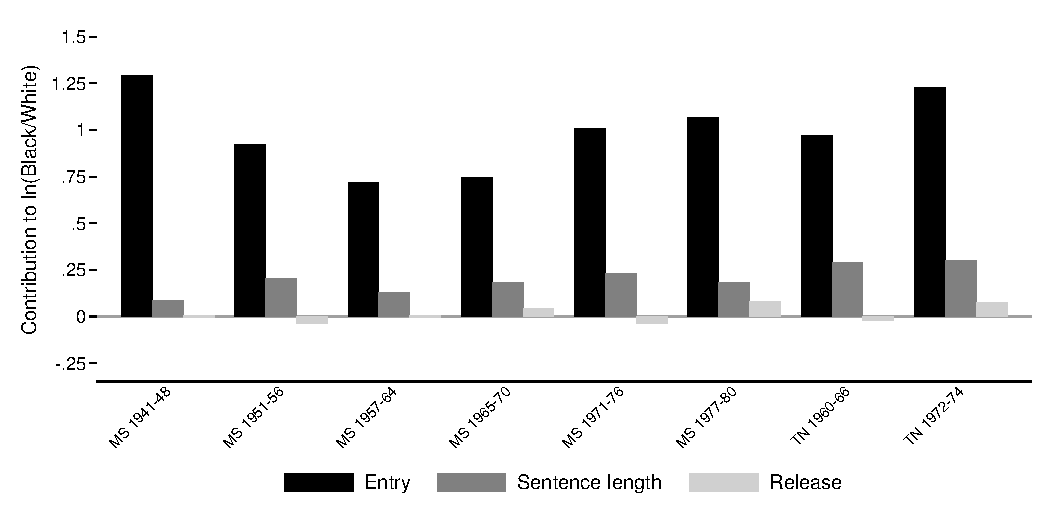
\includegraphics[ width=6.0in,  clip=true,  trim= 0.0in 0in 0in 0in ]{../../../30_output/40_figures/fig_decomp.pdf}
	\label{figure_decomp}
\end{center}
	\scriptsize{\emph{Notes:} Bars show the three terms of equation~\ref{equation_decomp} for each state and period (Table~\ref{table_decomp}).  Their sum is the log of the Black-White ratio of implied incarceration.  Release terms for MS 1971--76 and 1977--80 are unreliable because exits are under-observed.  }
\end{figure} \normalsize



The pattern over time in Mississippi is U-shaped.  The Black-White ratio in implied incarceration fell from 3.95\unskip~in 1941--48 to 2.97\unskip~in 1951--56 and 2.32\unskip~in 1957--64, before rising to 2.63\unskip~in 1965--70, 3.31\unskip~in 1971--76 and 3.78\unskip~in 1977--80.  Both the narrowing and the subsequent widening were driven by entry.  Through the 1950s, the narrowing reflected faster growth in White than in Black admission rates (Table~\ref{table_levels}).  After 1965, the widening reflected faster growth in Black admission rates.  From 1965--70 to 1971--76, the log gap increased by 0.23, of which the entry term contributed 0.26, the sentencing term 0.05, and the release term $-0.08$ (the latter unreliable owing to under-observed exits).  Tennessee's gap was larger than Mississippi's in the 1960s and grew further by 1972--74, again predominantly through entry.

The near-zero contribution of release is perhaps surprising, given the discretion that governed parole and clemency.  It does not, however, imply that release was race-neutral.  As I show below, it reflects two offsetting forces.





%% subsection
\subsection*{Comparing Like with Like: Within-County Differences}

\noindent The decomposition compares all Black and all White admissions in a state.  Racial differences in sentence length and release could reflect differences in offense, or the fact that Black and White prisoners were convicted in different counties with different courts.  To compare Black and White prisoners convicted in the same place and time, I estimate
\begin{equation}
	y_{icty} = \beta \, black_{i} + \gamma_{cy} + \pmb{X}_{i}'\delta + \varepsilon_{icty}
	\label{equation_within}
\end{equation}
where $y_{icty}$ is an outcome for admission $i$ convicted in county $c$ in year $y$, $\gamma_{cy}$ are county-by-year fixed effects, and $\pmb{X}_{i}$ includes fixed effects for the broad offense type (violent, property, drug, other), age, and sex (where recorded).  Standard errors are clustered by county of conviction.



% TABLE: Sentence
%---------------------------
\begin{table}[t!]\centering \footnotesize
\def\sym#1{\ifmmode^{#1}\else\(^{#1}\)\fi}
	\caption{Black-White differences in sentence length within county and year}\label{table_sentence}
	\smallskip
	\begin{tabular}{@{\extracolsep{5pt}}l*{6}{c}}
	\noalign{\smallskip}\noalign{\smallskip}\hline\hline\noalign{\smallskip}\noalign{\smallskip}
			&\multicolumn{6}{c}{$\ln$ effective sentence} \\
			\cline{2-7}  \noalign{\smallskip}
			                   &\multicolumn{1}{c}{(1)}         &\multicolumn{1}{c}{(2)}         &\multicolumn{1}{c}{(3)}         &\multicolumn{1}{c}{(4)}         &\multicolumn{1}{c}{(5)}         &\multicolumn{1}{c}{(6)}         \\
\midrule
Black           &     0.16\sym{***}&     0.17\sym{***}&    0.089\sym{***}&    0.097\sym{***}&     0.18\sym{***}&    0.026         \\
                &  (0.016)         &  (0.016)         &  (0.012)         &  (0.022)         &  (0.040)         &  (0.024)         \\
Black $\times$ Post-1965&                  &                  &                  &   -0.014         &                  &                  \\
                &                  &                  &                  &  (0.026)         &                  &                  \\
\midrule
State           &       MS         &       MS         &       MS         &       MS         &       TN         &       TN         \\
County $\times$ year FE&                  &\checkmark         &\checkmark         &\checkmark         &\checkmark         &\checkmark         \\
Offense type FE &                  &                  &\checkmark         &\checkmark         &                  &\checkmark         \\
Age and sex FE  &                  &                  &\checkmark         &\checkmark         &                  &\checkmark         \\
Observations    &    28268         &    27935         &    27926         &    27926         &    11492         &    11490         \\
 \\
	\noalign{\vspace*{-.17in}}\hline\hline\noalign{\smallskip}
\multicolumn{7}{p{5.6in}}{\scriptsize  \emph{Notes}: The above table presents OLS estimates of equation~\ref{equation_within}.  The sample is White and Black admissions, 1941--1980, with a parsed non-life, non-death effective sentence (top-coded at 50 years).  Column 1 includes state-by-year fixed effects only.  Offense type is the keyword-classified type of the first-listed crime.  Standard errors clustered by county of conviction.  \sym{*} \(p<0.1\), \sym{**} \(p<0.05\), \sym{***} \(p<0.01\) }
\end{tabular}
\end{table}



Table~\ref{table_sentence} presents estimates for sentence length.  In Mississippi, Black prisoners' sentences were 16 log points longer than White prisoners' sentences in the same year (column 1), and 18 log points longer than those of White prisoners convicted in the same county and year (column 2).  Accounting for broad offense type, age and sex halves this difference, to 9 log points (column 3).  The difference was not larger after 1965 (column 4); the change in the sentencing margin was not the channel through which racial disparity grew.  In Tennessee, the within-county difference of 18 log points (column 5) is almost entirely accounted for by differences in offense type (column 6).



% TABLE: Release
%---------------------------
\begin{table}[t!]\centering \footnotesize
\def\sym#1{\ifmmode^{#1}\else\(^{#1}\)\fi}
	\caption{Black-White differences in release, holding the sentence fixed}\label{table_release}
	\smallskip
	\begin{tabular}{@{\extracolsep{5pt}}l*{4}{c}}
	\noalign{\smallskip}\noalign{\smallskip}\hline\hline\noalign{\smallskip}\noalign{\smallskip}
			&\multicolumn{2}{c}{$\ln$ years served} &\multicolumn{2}{c}{First exit is parole} \\
			\cline{2-3} \cline{4-5}  \noalign{\smallskip}
			                   &\multicolumn{1}{c}{(1)}         &\multicolumn{1}{c}{(2)}         &\multicolumn{1}{c}{(3)}         &\multicolumn{1}{c}{(4)}         \\
\midrule
Black           &    0.054\sym{***}&    0.031\sym{**} &   -0.056\sym{***}&   -0.034\sym{**} \\
                &  (0.018)         &  (0.013)         & (0.0092)         &  (0.014)         \\
\midrule
State           &       MS         &       TN         &       MS         &       TN         \\
Admission years &  1941-70         &  1960-74         &  1941-70         &  1960-74         \\
County $\times$ year FE&\checkmark         &\checkmark         &\checkmark         &\checkmark         \\
Sentence length FE&\checkmark         &\checkmark         &\checkmark         &\checkmark         \\
Offense, age, sex FE&\checkmark         &\checkmark         &\checkmark         &\checkmark         \\
Observations    &     9519         &    11299         &     9519         &    11299         \\
 \\
	\noalign{\vspace*{-.17in}}\hline\hline\noalign{\smallskip}
\multicolumn{5}{p{5.0in}}{\scriptsize  \emph{Notes}: The above table presents OLS estimates of equation~\ref{equation_within} with additional fixed effects for the effective sentence (in whole years, with sentences over 20 years pooled).  The sample is admissions with a recorded first exit, in registers that record release events, in cohorts in which at least 85\% of exits are recorded (Mississippi through 1970, Tennessee 1960--1974).  The White share whose first exit is parole is  24\unskip\% in Mississippi and  48\unskip\% in Tennessee.  Standard errors clustered by county of conviction.  \sym{*} \(p<0.1\), \sym{**} \(p<0.05\), \sym{***} \(p<0.01\) }
\end{tabular}
\end{table}



Table~\ref{table_release} turns to release.  Here I compare Black and White prisoners who were convicted in the same county and year, of the same offense type, \emph{and} who received the same sentence.  Within these cells, Black prisoners in Mississippi served 5.7 log points longer before their first exit (column 1), and were 5.4 percentage points less likely to leave on parole (column 3)---a reduction of more than a fifth relative to the White parole share.  In Tennessee, Black prisoners served 3.1 log points longer, and were 3.4 percentage points less likely to be paroled.

Why, then, does the release margin contribute nothing to the aggregate gap?  The fraction of a sentence that is served falls steeply as sentence length increases---in Mississippi, from around all of a one-year sentence to under half of a sentence of more than ten years---because prisoners with long sentences were paroled or pardoned relatively earlier in their terms.  Because Black prisoners received longer sentences, their aggregate fraction served is pulled down by this composition, offsetting the disadvantage they faced holding the sentence fixed.  The aggregate decomposition therefore understates the role of discretionary release in producing racial inequality, and it attributes to the sentencing margin some of what is, in practice, an interaction between sentencing and release.





%% subsection
\subsection*{Where Did Entry Grow?}

\noindent Since entry is the dominant margin, and the margin through which the post-1965 racial gap grew, I examine its composition in two ways: by the type of offense, and by the racial composition of the county of conviction.

Figure~\ref{figure_offense} presents the Black-White difference in admission rates by offense type.  In Mississippi, property and violent offenses each account for between two-fifths and a little over one-half of the Black-White difference in admission rates in every period.  After 1965, the difference grew in both categories in similar proportion: in 1977--80, property offenses accounted for  51\unskip\% of the gap and violent offenses  46\unskip\%.  Drug offenses accounted for essentially none of the gap in any period.  Through 1980, the growth in racial disparity in Mississippi admissions did not run through drug enforcement.\footnote{This does not speak to the period after 1980, which is the focus of accounts emphasizing the war on drugs \citep{Alexander:2012tj}.  Offense types are classified from keywords in the transcribed crime and may mis-classify some offenses; ``other'' includes public order and miscellaneous offenses.}  In Tennessee, the gap grew most in violent offenses between 1960--66 and 1972--74.



%  FIGURE: Offense
%--------------------------------------
\begin{figure}[t!]
	\begin{center}
	\caption{Black-White difference in admission rates by offense type}
	\small \smallskip
		\begin{minipage}{3.1in} \centering \scriptsize \emph{(a) Mississippi} \\
			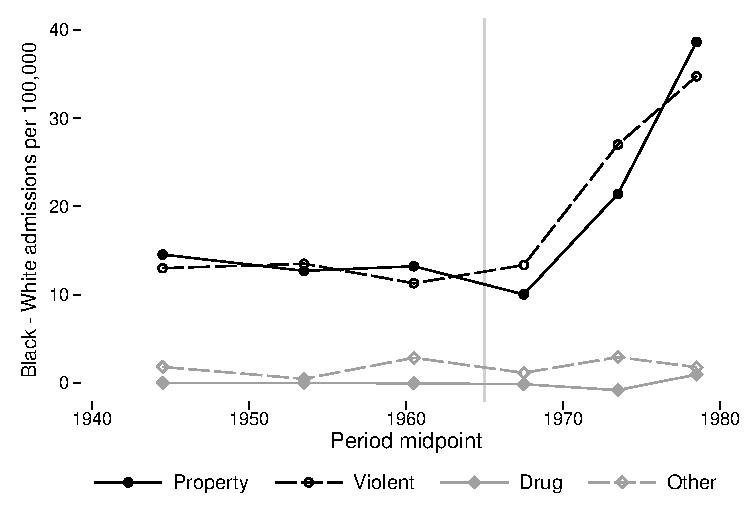
\includegraphics[ width=3.1in,  clip=true,  trim= 0.0in 0in 0in 0in ]{../../../30_output/40_figures/fig_offense_MS.pdf}
		\end{minipage}
		\begin{minipage}{3.1in} \centering \scriptsize \emph{(b) Tennessee} \\
			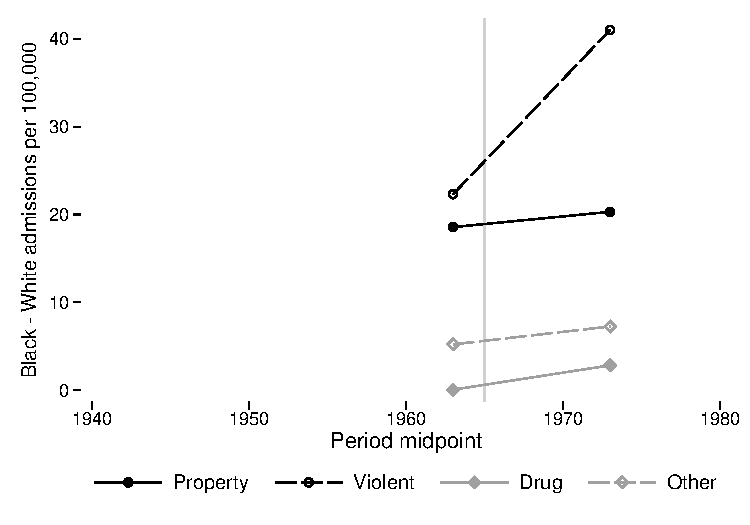
\includegraphics[ width=3.1in,  clip=true,  trim= 0.0in 0in 0in 0in ]{../../../30_output/40_figures/fig_offense_TN.pdf}
		\end{minipage}
	\label{figure_offense}
\end{center}
	\scriptsize{\emph{Source:} Convict registers; census population by race (interpolated). } \\
	\scriptsize{\emph{Notes:} Black minus White admissions per 100,000 residents of each race per year, by type of the first-listed offense, in the periods used in Table~\ref{table_decomp}, plotted at the period midpoint.  Admissions are scaled for coverage.  The vertical line marks 1965.  }
\end{figure} \normalsize



Figure~\ref{figure_county} presents admission rates by the racial composition of the county of conviction.  I divide Mississippi's counties into terciles by their Black population share in 1960.  Before 1965, Black admission rates were \emph{lowest} in the counties with the largest Black populations---a tercile that includes all of the plantation counties of the Delta---and highest in the counties with the smallest Black populations.  In the highest Black share counties, Black residents were admitted at 1.68\unskip~times the rate of White residents in 1957--64, compared to 2.60\unskip~times in the lowest tercile.  This is consistent with accounts in which the formal state prison was a less-used tool of racial control where private and local forms of control over Black labor were strongest \citep{Oshinsky:1997up,Muller:2019uv}.

After 1965, this pattern changed.  Black admission rates grew in every tercile, but the Black-White ratio grew most in the counties with the largest Black populations: from 1.34\unskip~in 1965--70 to 2.44\unskip~in 1971--76 and 2.78\unskip~in 1977--80.  In the lowest Black share tercile the ratio grew from 3.05\unskip~to 3.45\unskip.  The places in which the Voting Rights Act most threatened White political control are the places in which the racial gap in admissions widened most.  This accords with the state-level and county-level evidence in \cite{EubankFresh:2021gg}, and indicates that the channel was entry---the decisions of local police, prosecutors and courts---rather than sentencing or release.



%  FIGURE: County
%--------------------------------------
\begin{figure}[t!]
	\begin{center}
	\caption{Admission rates by the Black population share of the county of conviction, Mississippi}
	\small \smallskip
		\begin{minipage}{3.1in} \centering \scriptsize \emph{(a) Black admissions} \\
			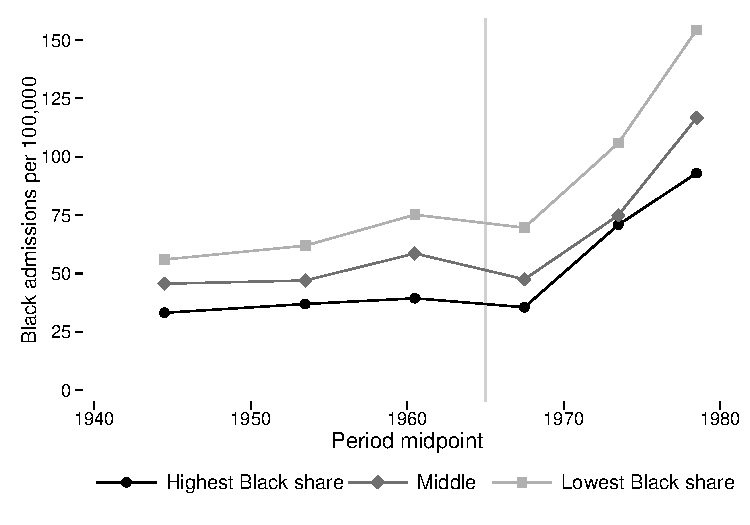
\includegraphics[ width=3.1in,  clip=true,  trim= 0.0in 0in 0in 0in ]{../../../30_output/40_figures/fig_county_black.pdf}
		\end{minipage}
		\begin{minipage}{3.1in} \centering \scriptsize \emph{(b) White admissions} \\
			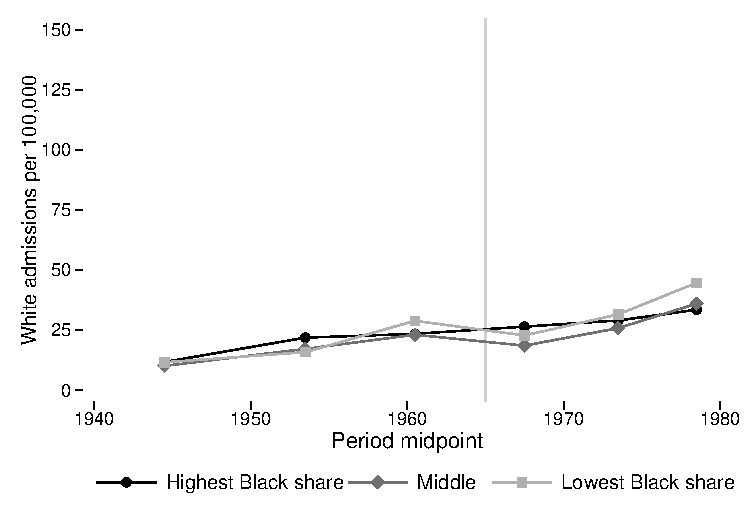
\includegraphics[ width=3.1in,  clip=true,  trim= 0.0in 0in 0in 0in ]{../../../30_output/40_figures/fig_county_white.pdf}
		\end{minipage}
	\label{figure_county}
\end{center}
	\scriptsize{\emph{Source:} Convict registers; census population by race (interpolated). } \\
	\scriptsize{\emph{Notes:} Admissions per 100,000 residents of each race per year, by tercile of the county's 1960 Black population share (terciles of Mississippi's counties), plotted at the period midpoint.  Only admissions matched to a county of conviction are included (more than 96\% in every period).  Admissions are scaled for coverage.  The vertical line marks 1965.  }
\end{figure} \normalsize







%----------------------------------SECTION-----------------------------------%
\vspace*{-.1in}
\section*{Discussion}
\vspace*{-.1in}

\noindent The results establish that racial inequality in incarceration in mid-century Mississippi and Tennessee was produced primarily at the point of entry.  This is important for three reasons.

First, it locates the production of racial inequality in incarceration at the most local, least visible, and least studied stage of the carceral process.  Admission to prison is the end-point of decisions by county sheriffs, police, prosecutors and judges---many of them locally elected.  In the mid-century South, these were the offices through which local White political control was exercised \citep{Mickey:2015vh}.  That the post-1965 widening of the racial gap was concentrated in high Black share counties, and in the entry margin, is consistent with these offices responding to the threat that Black enfranchisement posed to that control \citep{EubankFresh:2021gg}.

Second, the results qualify accounts that place drug policy and sentencing law at the center of the origins of racial disparity in incarceration.  In Mississippi, neither drug offenses nor changes in the racial gap in sentence length account for the growth in disparity before 1980.  These accounts may well explain the further growth of incarceration after 1980 \citep{Alexander:2012tj,Pfaff:2017tp}, but the racial gap in imprisonment was already widening, through entry for property and violent offenses, before the war on drugs.

Third, the results caution against concluding from aggregate data that a margin is race-neutral.  The aggregate release margin contributes nothing to the racial gap.  Yet, comparing like with like, Black prisoners in Mississippi served longer for the same sentence and were less likely to be paroled.  Discretionary release disadvantaged Black prisoners, but this was masked in aggregate by their longer sentences.

There are two broad categories of bias---indeed, racism---that might produce these disparities.  The first is institutional, a function of broad rules and the unequal circumstances to which they are applied, rather than individual decision-making.  The second is individual, the discretionary decisions of police, prosecutors, judges, juries and parole boards.  The registers cannot distinguish between them.  The entry disparities, in particular, combine differences in offending with differences in enforcement and prosecution, and I do not observe the population at risk of arrest.  The within-county comparisons of sentence and release hold constant the court, year, offense type and sentence, but not the details of the offense or the prisoner's record, which may differ by race.  At the same time, the prisoner's record may itself be the product of earlier discretionary decisions, so that controlling for it would understate disparity \citep{Tonry:2011hh}.

The analysis has further limitations.  The implied stock is a steady-state construct: the observed prison population also reflects the accumulated admissions of earlier years and the life-sentenced population, which the decomposition excludes.  Release is measured from registers that were not always updated, so that the release margin is unreliable for Mississippi cohorts admitted after 1970.  And Mississippi and Tennessee are two states.  Whether the same margins produced racial inequality elsewhere---in the North, where \cite{Muller:2012wf} documents earlier growth in racial disparity, or in Sunbelt states where the punitive turn has been traced \citep{Lynch:2010rt,Schoenfeld:2018vq}---is an open question.







%----------------------------------SECTION-----------------------------------%
\vspace*{-.1in}
\section*{Conclusion}
\vspace*{-.1in}

\noindent In this article, I study how racial inequality in incarceration was produced in the mid-20th century U.S. South, using new individual-level data on the universe of admissions to the Mississippi state penitentiary from 1941 to 1981, and on admissions to Tennessee's prisons in the 1960s and early 1970s.

I find that the entry margin---who is admitted to prison---accounts for the large majority of the racial gap in incarceration in every period, with longer sentences for Black prisoners accounting for most of the remainder.  The racial gap in Mississippi narrowed through the 1950s and widened after 1965.  That widening came through entry, was concentrated in counties with the largest Black populations, and ran through property and violent offenses rather than drug offenses.  Within the same county and year, Black prisoners received longer sentences and, holding the sentence fixed, served longer and were less likely to be paroled.

These results are not a causally identified test of a single explanation for the growth of racial disparity in incarceration.  But they document where in the carceral process that disparity was produced, and how that changed across the end of Jim Crow---facts any explanation must account for.  That the margin that mattered most was the one governed by local officials, and that it changed most where Black political power grew most, suggests that the political economy of local criminal justice institutions deserves a central place in accounts of how the U.S. came to incarcerate its Black citizens at such disproportionate rates.  The consequences of that incarceration for Black political participation and citizenship \citep{Uggen:2002th,Manza:2008vp,Burch:2014ug,Lerman:2014wr} suggest, in turn, that the margins of incarceration are not only an outcome of politics, but an input into it.






%------------------------------ SECTION -----------------------------------%
\vspace*{.6in}
\singlespacing
\textbf{Research Assistants:} Eleanor Ross, David Marin, Chris Liang, Lilly Ma, Jacqueline Perez, Ryan Mitchell, Drew Greene, Brooke Bowen, Sarai Chaidez, Connor Booher, Sanya Uppal, Madison Lee, Maya Regal, Saralyn Carcy, Gai Chintala, Cynthia Dong, Hannah Lawry, Cydney Livingston, Malenie Reyes, Satya Khurana, Colleen Siv, Brynn Meyercord, Esme Gova, Evelyn Shi, Rashad Rahman, Mia Meier, Sachin Shah, Nick Haddad, Vaneesha Patel, Adriana DeLorenza, Briana Cellini, Breanna Collins, Cat Xia, Ellie Siebeneck, Karen Ru, Lexi Jackson, Jonah Perrin, Sanceray Smith, Jamie Lim, James McIntyre, Darshan Vijaykumar, Olivia Kramer, Brianna Joyce, Jeff Du, Kamdon Early, and Kris Zhu.  Thank you.  Without your help, this research simply could not have happened.




%------------------------------- REFERENCES --------------------------------%

\clearpage \newpage
\singlespacing
\bibliographystyle{apsr}
\bibliography{/Users/Vesper/Documents/Bibtex/Complete_Library.bib}







%------------------------------- APPENDIX --------------------------------%
\clearpage \newpage
\appendix
\onehalfspacing
\setcounter{table}{0}
\renewcommand{\thetable}{A\arabic{table}}
\setcounter{figure}{0}
\renewcommand{\thefigure}{A\arabic{figure}}

\begin{center}
	\section*{\normalfont \LARGE Appendix to \\``The Margins of Mass Incarceration''}
\end{center}



%% section
\section{Constructing the Register Data}\label{appendix_data}

\noindent The Mississippi registers are organized in lettered books, each divided into numbered parts for transcription.  The professional transcriptions and the student transcriptions were delivered as separate spreadsheets for each part (or range of parts).  I combine them as follows.

\emph{Duplicates and misfiled parts.}  Several parts were transcribed twice, and several spreadsheets were labelled with the wrong book or part.  I identify these by comparing the content of each part's transcribed records (age, county, sentence date, term and race) across files.  Where a part's records duplicate those of another part, I keep the correctly labelled copy and drop the duplicate.  Where a part was transcribed by both a professional and a student transcriber, I keep the professional transcription.  Two professionally transcribed parts proved to be copies of other parts (one re-typed, and one with day and month transposed in every date); as a result, the true content of these two parts has not yet been transcribed.

\emph{Dates.}  Dates are parsed from the transcribed text.  In approximately 550 professionally transcribed records, the received date has day and month transposed, which I identify where the transposed date falls between 0 and 120 days after the date of sentence while the date as written does not.  I correct these and flag them.  Where the received date is missing, I use the date of sentence.

\emph{Release events.}  Release events are parsed from the discharge, parole and pardon columns using keywords and dates.  The instructions given to student transcribers described parole entries as not essential, and some student files recorded only final discharges.  I therefore measure release only in files in which release events are recorded.

\emph{Counties and offenses.}  Counties of conviction are matched to a canonical list of county names after correcting transcription misspellings; unclear strings are left unmatched rather than guessed.  Offenses are classified into violent, property, drug and other offense types using keywords in the first-listed crime.



%% section
\section{Coverage}\label{appendix_coverage}

\noindent For Mississippi, I measure the share of each year covered by the transcribed register pages by ordering the parts chronologically, dating each part by the median admission date of its records, and computing the share of each year's parts that are transcribed, multiplied by the share of the year for which register images survive.  For Tennessee, coverage is the share of each calendar year within the date spans of the transcribed microfilm rolls.  Figure~\ref{figure_coverage} presents coverage by year.



%  FIGURE: Coverage
%--------------------------------------
\begin{figure}[h!]
	\begin{center}
	\caption{Share of each year's register transcribed}
	\small \smallskip
		\begin{minipage}{3.1in} \centering \scriptsize \emph{(a) Mississippi} \\
			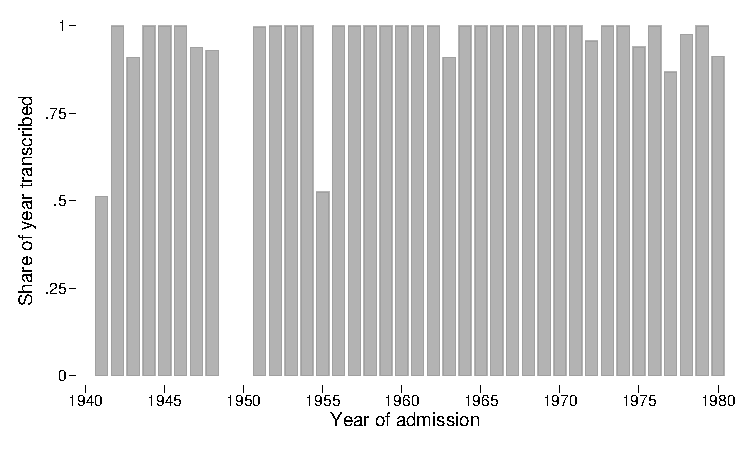
\includegraphics[ width=3.1in,  clip=true,  trim= 0.0in 0in 0in 0in ]{../../../30_output/40_figures/fig_coverage_MS.pdf}
		\end{minipage}
		\begin{minipage}{3.1in} \centering \scriptsize \emph{(b) Tennessee} \\
			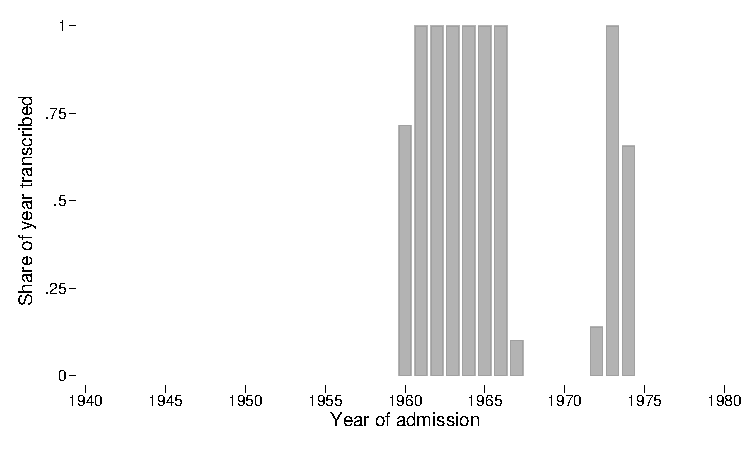
\includegraphics[ width=3.1in,  clip=true,  trim= 0.0in 0in 0in 0in ]{../../../30_output/40_figures/fig_coverage_TN.pdf}
		\end{minipage}
	\label{figure_coverage}
\end{center}
	\scriptsize{\emph{Notes:} Mississippi: no register images survive for November 1948 to December 1950.  Tennessee: microfilm rolls covering 1967--1972 are not among the images, and rolls after August 1974 are not transcribed.  }
\end{figure} \normalsize



%% section
\section{Validation Against Published Admission Counts}\label{appendix_validate}

\noindent Table~\ref{table_validate} compares admissions in the registers to the admissions reported in the states' published reports \textbf{[TK: citation for the annual report series]}.



% TABLE: Validation
%---------------------------
\begin{table}[h!]\centering \footnotesize
	\caption{Register admissions compared to published admission counts}\label{table_validate}
	\smallskip
	\begin{tabular}{@{\extracolsep{5pt}}ll*{6}{c}}
	\noalign{\smallskip}\noalign{\smallskip}\hline\hline\noalign{\smallskip}\noalign{\smallskip}
			& & & \multicolumn{3}{c}{Admissions} & \multicolumn{2}{c}{Black share} \\
			\cline{4-6} \cline{7-8} \noalign{\smallskip}
			State & Year & Coverage & Report & Register & Ratio & Report & Register \\
	\noalign{\smallskip}\hline\noalign{\smallskip}
			   Mississippi & 1960 &   1.00 &       854 &       862 & 1.01 & 0.61 & 0.62 \\
Mississippi & 1964 &   1.00 &       793 &       841 & 1.06 & 0.60 & 0.59 \\
Mississippi & 1970 &   1.00 &       666 &       739 & 1.11 & 0.56 & 0.54 \\
Mississippi & 1975 &   0.94 &     1,248 &     1,254 & 1.00 & 0.64 & 0.63 \\
Mississippi & 1976 &   1.00 &     1,053 &     1,320 & 1.25 & 0.65 & 0.64 \\
Mississippi & 1979 &   1.00 &     1,791 &     1,790 & 1.00 & 0.59 & 0.59 \\
Mississippi & 1980 &   0.91 &     3,600 &     1,658 & 0.46 & 0.46 & 0.64 \\
\noalign{\smallskip}
Tennessee & 1962 &   1.00 &     1,212 &     1,269 & 1.05 & -- & -- \\
Tennessee & 1965 &   1.00 &     1,320 &     1,503 & 1.14 & -- & -- \\
Tennessee & 1966 &   1.00 &     1,424 &     1,264 & 0.89 & -- & -- \\
Tennessee & 1967 &   0.10 &     1,215 &       117 & 0.10 & -- & -- \\
Tennessee & 1972 &   0.14 &     1,527 &       200 & 0.13 & -- & -- \\
Tennessee & 1973 &   1.00 &     1,432 &     1,541 & 1.08 & -- & -- \\
Tennessee & 1974 &   0.66 &     1,617 &     1,219 & 0.75 & -- & -- \\
 \\
	\noalign{\vspace*{-.17in}}\hline\hline\noalign{\smallskip}
\multicolumn{8}{p{5.4in}}{\scriptsize  \emph{Notes}: \emph{Register} is the number of transcribed admissions (not scaled for coverage).  \emph{Coverage} is the share of the year's register transcribed; register counts in years with low coverage (Tennessee 1967 and 1972) are not comparable to the report.  Black shares are compared for Mississippi only. }
\end{tabular}
\end{table}




%----------------------------- END DOCUMENT -------------------------------------%
\end{document}
